\documentclass[11pt]{article}

% ===================== PACKAGES =====================
\usepackage[margin=1in]{geometry}     % 1-inch margins
\usepackage{mathptmx}                  % Times New Roman font
\usepackage{setspace}                  % Double spacing
\usepackage{amsmath, amssymb, amsthm}
\usepackage{bm}
\usepackage{graphicx}
\usepackage{booktabs}
\usepackage{array}
\usepackage{xcolor}
\usepackage{hyperref}
\usepackage{titlesec}
\usepackage{enumitem}
\usepackage{caption}

\hypersetup{
    colorlinks=true,
    linkcolor=blue!50!black,
    citecolor=blue!50!black,
    urlcolor=blue!50!black,
}

% Section formatting
\titleformat{\section}{\normalfont\large\bfseries}{\thesection.}{0.5em}{}
\titleformat{\subsection}{\normalfont\normalsize\bfseries}{\thesubsection.}{0.5em}{}

\pagenumbering{arabic}
\sloppy
\doublespacing

% Math operators
\DeclareMathOperator*{\argmax}{arg\,max}
\DeclareMathOperator*{\argmin}{arg\,min}

% ===================== TITLE =====================
\title{\vspace{-2em}\textbf{How to Eat Mushrooms in the Wild Without Getting Killed:\\
Active Learning for Fungal Edibility Classification}}
\author{Luci Lu \and Ziyan Zhang}
\date{}

% ===================== DOCUMENT =====================
\begin{document}

\maketitle
\thispagestyle{plain}

% =====================================================
% 1. BACKGROUND
% =====================================================
\section{Background}

\subsection{Fine-Grained Fungal Image Classification}

Eating wild mushrooms is a popular activity and a small industry in many parts
of the world, but every year thousands of people end up in the hospital
because they mistook a poisonous species for an edible one. There are more
than $14{,}000$ known mushroom species, and many of them look almost the same even though one is safe and the other is not. The most famous example is the
Amanita phalloides (Death Cap), which can kill a person but looks
similar to several edible Agaricus mushrooms. This issues make mushroom classification a good test case for machine
learning methods that care about safety and not only accuracy. The mushrooms
look alike, calling a toxic one ``safe'' is much worse than the other way
around, and some species have far more photos than others.

The Danish Fungi 2020 (DF20) benchmark from Picek et al.~[1] is one of the
best public datasets we found for this task. The images come from the Atlas
of Danish Fungi, where people submit photos of mushrooms they have seen.
DF20 has a few nice properties for our work. The species labels are checked
against the official taxonomy, each photo comes with extra information like
location and habitat. The last
point matters because it means we can use ImageNet-pretrained models without
worrying that the model has already seen the test images. In their paper,
Picek et al.\ trained a Vision Transformer (ViT-B/16-224) on DF20 and got
about $0.72$ top-1 species accuracy and $0.74$ macro F1. The same group later released a smaller version called DF20-Mini, which
keeps only the species that have enough images to train on. This makes
DF20-Mini more suitable for machine learning, since every class has a
reasonable number of training examples instead of just one or two, which can be used as a backbone for other tasks.

A related line of work by Picek et al.~[2] used a similar model in the
FungiVision citizen-science app, which shows that large-scale mushroom
recognition can actually work in practice when there is enough labeled data
to train on. Our project looks at the opposite situation, that is,  what can we
do when labeled data is scarce.

\subsection{Active Learning Speeds Up the Labeling Process}

Active learning (AL) is a way of training a model where, instead of labeling
all the data at once, the model picks which examples it wants labeled next.
The idea is to reach a good accuracy with fewer total labels than you would
need if you just picked images at random~[3]. Suppose we have a labeled set
$L$, an unlabeled pool $U$, a model with parameters $\theta$, and we are
allowed to label $B$ new examples each round. An AL strategy is a scoring
function $a(\cdot)$ that picks the best batch of $B$ examples from the
unlabeled pool,
\[
Q \;=\; \argmax_{Q \subseteq U,\ |Q| = B}\ a(Q;\,\theta, L, U).
\]
After labeling these examples, we add them to the labeled set,
$L \leftarrow L \cup Q$, and retrain the model. This loop repeats until the
labeling budget runs out.

There are several common families of AL strategies, and each one has a
different idea about what makes an example worth labeling. Uncertainty
sampling picks examples that the current model is least sure about.
Diversity sampling picks examples that look different from what is already
in the labeled set, so the labeled data covers more of the feature
space~[4]. Bayesian methods like BALD~[5] try to find the examples that
would teach the model the most, by separating the part of the uncertainty
that comes from the model itself from the part that comes from noise in the
data. Class-balanced methods add a weighting term that pushes the model to
ask for more examples of rare classes, which helps a lot on long-tailed
datasets~[7].


\subsection{From Species Prediction to Edibility Prediction}

When someone is out in the woods picking mushrooms, they do not really need
to know the exact species. What they need to know is whether the mushroom is
safe to eat. So instead of stopping at species-level prediction, a four-way edibility decision is prefered. The four buckets are SAFE
(edible raw or cooked), COOK\_FIRST (only safe after proper cooking), AVOID
(toxic, deadly, or just inedible), and UNCERTAIN (the literature does not
agree, or there is not enough information).

It is important to note that the four buckets are not the training target.
The model is still trained on all $179$ species, and we only convert the
species prediction into a bucket prediction at the end. Let $g$ be the
function that maps each species $c$ to its bucket $k$, so
$g:\{1,\ldots,C\}\to\{1,\ldots,K\}$. There are two natural ways to do this
conversion. The first is hard decoding, where we first take the most likely
species and then look up its bucket,
\begin{align}
\hat b_{\text{hard}}(x) &\;=\; g\!\left(\argmax_{c}\ p(y=c\mid x)\right).
\label{eq:hard}
\end{align}
The second is soft decoding, where we add up the predicted probabilities of
all species inside each bucket and pick the bucket with the largest total,
\begin{align}
\hat b_{\text{soft}}(x) &\;=\; \argmax_{k}\ \sum_{c:\,g(c)=k} p(y=c\mid x).
\label{eq:soft}
\end{align}
The nice thing about Equation~\eqref{eq:soft} is that it forgives mistakes
between species that share a bucket. For example, if the model is confused
between two edible \emph{Boletus} species, the bucket prediction can still
come out right. We test whether this actually helps in our experiments.
% =====================================================
% 2. SIGNIFICANCE
% =====================================================
\section{Significance}

Most fine-grained image classification work focuses on getting the highest
top-1 accuracy and treats every error the same way. But in a real foraging
setting, the cost of errors is not even. Mistaking a Death Cap for an
edible Agaricus can kill people, while mixing up two edible
Russula species does not really matter. We handle this in two ways. First, instead of stopping at the species prediction, we group the $179$ species into four edibility buckets and check how well the model does on those buckets. Second, on top of the usual
accuracy numbers, we also report the recall for each bucket, so we can see
how often the model misses the toxic ones. This way, the evaluation matches
what a real user would care about. 

The active learning literature has lots of strategies, but it is not very
clear which one to use for a fine-grained, long-tailed, safety-critical task
like ours. We compare six strategies across five seeds and report six
different metrics, including bucket accuracy, macro F1, and per-bucket
recall. As far as we know, this is the first benchmark of this kind on
DF20-Mini. One thing we found is that the ranking of strategies changes a
lot depending on the metric. For example, BALD could be the best on overall bucket accuracy,
but class-balanced entropy may be much better at catching the UNCERTAIN class.
This kind of trade-off matters for any AL deployment where the metric the
user cares about is not the same as the loss the model was trained on.

Annotation is also the bottleneck for extending mushroom recognition beyond
Denmark. Labeling fungal images requires expert mycologists, and they are
hard to find. So cutting the labeling cost is not just a nice engineering
result, it is what makes it realistic to build similar systems for new
regions or for rare species, where the safety benefit is the largest. To show how much labeling effort active learning can save, we compare each
strategy against a full-supervision ceiling, where the model is trained on
the entire labeled pool. This suggests that a usable safety-aware
classifier for a new region could be built with a manageable annotation
budget.

% =====================================================
% 3. SPECIFIC AIMS
% =====================================================
\section{Specific Aims}

The overall goal of this project is to find out whether modern active
learning strategies can build a useful, safety-aware mushroom classifier
without needing too many labels, by mapping images into the four edibility
buckets defined earlier. We further break this down into three smaller aims.

\paragraph{Aim 1. Build an edibility label hierarchy on top of the species
labels.}
We use a large language model (Claude Opus~4.7) to assign each of the $179$
DF20-Mini species to one of four edibility buckets. Then we check whether
the resulting hierarchy makes sense by looking at how the buckets are split
across the six genera, how balanced the buckets are at the image level, what
kinds of toxicity end up inside the AVOID bucket, and how confident the LLM
was for each bucket. The output is an enriched label table that supports both
species-level training and bucket-level evaluation through Equations
\eqref{eq:hard} and \eqref{eq:soft}.

\paragraph{Aim 2. Build an active learning pipeline using 
embeddings data.}
We extract $768$-dimensional embeddings from the ViT-B/16-224 backbone
released by Picek et al.~[1], which was already fine-tuned on DF20-Mini. On
top of these embeddings, we train a small MLP head with MC-dropout,
and run a low-budget AL loop with $N_{\text{init}}=400$ initial labels, a
batch size of $B=100$ per round, and a total budget of $5{,}000$ labels.
We then compare six query strategies (random, entropy, margin, core-set,
class-balanced entropy, and BALD) using five random seeds, and we also train
a fully supervised model on the entire pool to get an upper bound.

\paragraph{Aim 3. Evaluate the strategies.}
We report species accuracy, species macro F1, bucket accuracy under both
hard and soft decoding, per-bucket recall, and a Pareto plot of overall
accuracy against UNCERTAIN recall. We also measure label efficiency by
counting how many labels each strategy needs to reach $80\%$, $90\%$, and
$95\%$ of the full-supervision ceiling. Finally, we run a per-genus analysis
with extra attention to the genus Amanita, which contains the most
dangerous species in the dataset.


% =====================================================
% 4. EXPERIMENTAL DESIGN
% =====================================================
\section{Experimental Design}

\subsection{Dataset and Label Hierarchy}

We use DF20-Mini~[1] with its official train and test split. After dropping
the rows with missing species labels, the training pool has about $32{,}724$
images and the test set has about $4{,}000$ images. Together they cover
$C=179$ species across $6$ genera (\emph{Amanita}, \emph{Boletus},
\emph{Russula}, \emph{Mycena}, \emph{Agaricus}, and \emph{Clitocybe}).

To get the edibility labels, we ask Claude Opus~4.7 about each species and
have it return both an edibility label and a confidence rating in
$\{\text{high}, \text{medium}, \text{low}\}$. We then map the LLM output
into one of the $K=4$ buckets using the rule
\[
g(\text{species}) =
\begin{cases}
\text{SAFE} & \text{if the LLM label is } \text{edible},\\
\text{COOK\_FIRST} & \text{if the LLM label is } \text{edible\_cooked\_only},\\
\text{AVOID} & \text{if the LLM label is one of } \{\text{poisonous, deadly, inedible}\},\\
\text{UNCERTAIN} & \text{if the LLM label is } \text{unknown}.
\end{cases}
\]
At the image level, this gives us roughly $12\%$ SAFE, $20\%$ COOK\_FIRST,
$55\%$ AVOID, and $13\%$ UNCERTAIN, which is much more balanced than the
$179$-way species distribution where the most common species has about
$39$ times more images than the rarest one.

\subsection{Backbone and Embedding Extraction}

To keep our experiments focused on the AL strategy rather than on
representation learning, we use a frozen feature extractor. We take the
public DF20M ViT-B/16-224 checkpoint from Picek et al.~[1] and remove the
classification head, then run every DF20-Mini image through the backbone to
get a $d = 768$-dimensional embedding,
\[
\phi:\ \mathbb{R}^{3 \times 224 \times 224} \;\to\; \mathbb{R}^{768},
\qquad
\tilde\phi(x) \;=\; \phi(x) / \|\phi(x)\|_2.
\]
We $\ell_2$-normalize the embeddings so that cosine similarity is
well-defined, which is needed by the core-set strategy. As a sanity check,
fitting a logistic regression on $\tilde\phi(x)$ gives roughly the same
species accuracy that Picek et al.\ report, which tells us the checkpoint
loaded correctly. 

\subsection{The MC-Dropout MLP Classifier}

The classifier head $f_\theta : \mathbb{R}^{768} \to \Delta^{C-1}$ is a
small MLP,
\[
f_\theta = \text{Linear}_{768 \to 512} \to \text{ReLU} \to \text{Drop}_p
\to \text{Linear}_{512 \to 256} \to \text{ReLU} \to \text{Drop}_p
\to \text{Linear}_{256 \to 179},
\]
with dropout probability $p = 0.4$. Following Gal and Ghahramani~[6], we
keep dropout turned on at inference time, so $T = 20$ stochastic forward
passes give us $T$ slightly different predictions
$\{p(y \mid x, \theta_t)\}_{t=1}^{T}$ that act like samples from an
approximate posterior. These are what BALD needs.

First, we retrain the head from
scratch every AL round instead of fine-tuning it from the previous round.
We tried the warm-start version and saw that the BALD scores got biased
toward the dropout masks that happened to be active in the previous
training, so retraining from scratch is the cleaner option. Second, we use
two hidden layers with $p = 0.4$. With only one hidden layer, the model
becomes too confident on the small early labeled sets and BALD stops working
properly. Training uses AdamW with learning rate $10^{-3}$, weight decay
$\lambda = 5 \times 10^{-4}$, batch size $128$, and $30$ epochs, with the
cross-entropy loss
\[
\mathcal{L}(\theta) \;=\; -\frac{1}{|L|} \sum_{(x,y) \in L}
\log p(y \mid x, \theta) \;+\; \tfrac{\lambda}{2} \|\theta\|_2^2.
\]
We picked these hyperparameters by checking train and test accuracy every
five epochs to see when the model converged.

\subsection{Active Learning Loop}

We use a low-budget AL setup that mimics a realistic labeling project where
expert time is the bottleneck.

\textbf{Initial labeled set.} We start with $N_{\text{init}} = 400$ labeled
images, drawn by stratified sampling so that each of the $179$ species gets
about $2$ examples. This avoids the cold-start problem where some classes
are never seen by the model in the first few rounds.

\textbf{Batch size and total budget.} At each round, the strategy picks
$B = 100$ new images to label. The loop stops once the labeled set reaches
$5{,}000$ images, which is about $15\%$ of the full training pool.

\textbf{Per-round procedure.} In each round, we retrain the MLP head from
scratch on the current labeled set, evaluate it on the held-out test set,
and use the trained model to score the unlabeled pool. The top $B = 100$
images are then added to the labeled set for the next round.

\textbf{Seeds and reporting.} We repeat each strategy with five random
seeds and report the mean learning curve, with the $\pm 1$ standard
deviation across seeds shown as a shaded band. As an upper bound, we also
train the same MLP head on the entire training pool to get a
full-supervision ceiling.
\subsection{Query Strategies}

We compare six strategies in total, covering the four families described in
the Background.

\textbf{Random.} The passive baseline. Each round it samples $B$ examples
uniformly from the unlabeled pool, $Q_r \sim \text{Uniform}(U_r)$.

\textbf{Entropy.} Picks the top $B$ examples by predictive entropy,
\[
H[p(y \mid x)] \;=\; -\sum_{c=1}^{C} p(y = c \mid x) \log p(y = c \mid x).
\]
Entropy is high when the model spreads its probability across many classes,
so this strategy goes after the examples the model is least sure about.

\textbf{Margin.} Picks the bottom $B$ examples by the gap between the
top two predicted probabilities,
\[
m(x) \;=\; p_{(1)}(x) - p_{(2)}(x).
\]
A small $m(x)$ means the model is torn between two classes, so this
strategy targets borderline cases.

\textbf{Core-set~[4].} A diversity-based method. It picks the example that
is farthest from anything we have already labeled, using one minus cosine
similarity in the embedding space,
\[
x^{*} \;=\; \argmax_{x \in U}\ \min_{x' \in L}\ d(\tilde\phi(x), \tilde\phi(x')),
\qquad
d(x, x') = 1 - \tilde\phi(x)^{\top} \tilde\phi(x').
\]
We pick $B$ samples greedily, updating the minimum distance after each
selection.

\textbf{Class-balanced entropy~[7].} A long-tail-aware version of entropy.
We multiply the entropy score by a class-frequency weight that is bigger for
classes we have seen less,
\[
w_c \;=\; \frac{1}{\sqrt{n_c + 1}},
\qquad
x^{*} \;=\; \argmax_{x \in U}\ H[p(y \mid x)] \cdot w_{\hat y(x)},
\]
where $n_c$ is how many examples of class $c$ are already in the labeled
set and $\hat y(x)$ is the model's predicted class for $x$.

\textbf{BALD~[5].} A Bayesian strategy. We approximate the BALD score
with $T = 20$ MC-dropout forward passes,
\[
\widehat{\text{BALD}}(x)
\;=\; H\!\left[\tfrac{1}{T} \sum_{t=1}^{T} p(y \mid x, \theta_t)\right]
\;-\; \tfrac{1}{T} \sum_{t=1}^{T} H\!\left[p(y \mid x, \theta_t)\right],
\]
which approximates the part of the model's uncertainty that comes from the
model itself rather than from noise in the data. The strategy picks the
top $B$ samples by this score.

For comparison, we also train the same MLP on the entire labeled pool
($L = U$) to get a full-supervision ceiling.

\subsection{Evaluation Metrics}

For each (strategy, seed, round) triple, we record six headline numbers.
These are species top-1 accuracy, species macro F1, bucket accuracy under
both hard and soft decoding (Equations~\eqref{eq:hard} and \eqref{eq:soft}),
bucket macro F1 under both schemes, and per-bucket recall,
\[
\text{Recall}_k \;=\;
\frac{|\{i : \hat b(x_i) = k,\ b(x_i) = k\}|}
     {|\{i : b(x_i) = k\}|}.
\]
We also store per-genus species accuracy, so we can later check how much of
the headline performance comes from each genus.

\paragraph{Label efficiency.} For each target $\tau \in \{0.80,\,0.90,\,0.95\}$
and each strategy, we find the smallest budget at which the strategy crosses
$\tau$ times the full-supervision accuracy,
\[
N_\tau(\text{strategy}) \;=\; \min\bigl\{n :
\text{acc}_{\text{strategy}}(n) \ge \tau \cdot \text{acc}_{\text{full-sup}}\bigr\}.
\]
If a strategy fails to reach the target inside the $5{,}000$-label budget
for a particular seed, that seed is left out of the mean and we report the
success rate (for example $4/5$) alongside the number.

\subsection{Safety-Focused Analysis}

On top of the headline numbers, we run three extra analyses that focus on
the safety side of the problem. First, we plot AVOID recall and UNCERTAIN
recall as their own learning curves. The AVOID curves end up tightly
clustered, which means toxic species are caught reliably no matter which
strategy we use. The UNCERTAIN curves are much more spread out, which
suggests that the choice of strategy matters most when the goal is flagging
ambiguous specimens. Second, we make a Pareto plot of bucket accuracy
against UNCERTAIN recall at the final budget. BALD is the best on overall
accuracy but drops to fifth on UNCERTAIN recall, while class-balanced
entropy goes the other way. Third, we build a per-genus heatmap of bucket
recall. The lethal genus \emph{Amanita} reaches an AVOID recall of $0.89$
even when the species accuracy is only around $0.65$, which shows the
benefit of the soft-aggregation decoder in Equation~\eqref{eq:soft}.


% =====================================================
% 5. RESULTS
% =====================================================
\section{Results}

We present the results in the same order as the three specific aims:
the LLM-derived edibility hierarchy (Aim~1), the embedding-quality sanity
check and the full-supervision ceiling (Aim~2), and the head-to-head
comparison of the six AL strategies (Aim~3). All AL numbers are reported
as the mean across five seeds, with $\pm 1$ standard deviation in
parentheses where space allows.

\subsection{The Edibility Hierarchy is Balanced and Epistemically Coherent}

Mapping the $179$ DF20-Mini species through the LLM and the rule in
Section~4.1 yields $21$ SAFE species ($11.7\%$), $37$ COOK\_FIRST ($20.7\%$),
$96$ AVOID ($53.6\%$), and $25$ UNCERTAIN ($14.0\%$). At the image level
the picture flattens to $15.0\%$ / $21.0\%$ / $57.0\%$ / $7.0\%$ across the
$36{,}361$ images (Figure~\ref{fig:bucket-pie}). Compared with the raw
$179$-way distribution, where the most populated species has roughly $39\times$
the support of the rarest, the four-bucket view is far more tractable for
classification while still preserving the safety semantics that motivate the
project.

\begin{figure}[h]
\centering
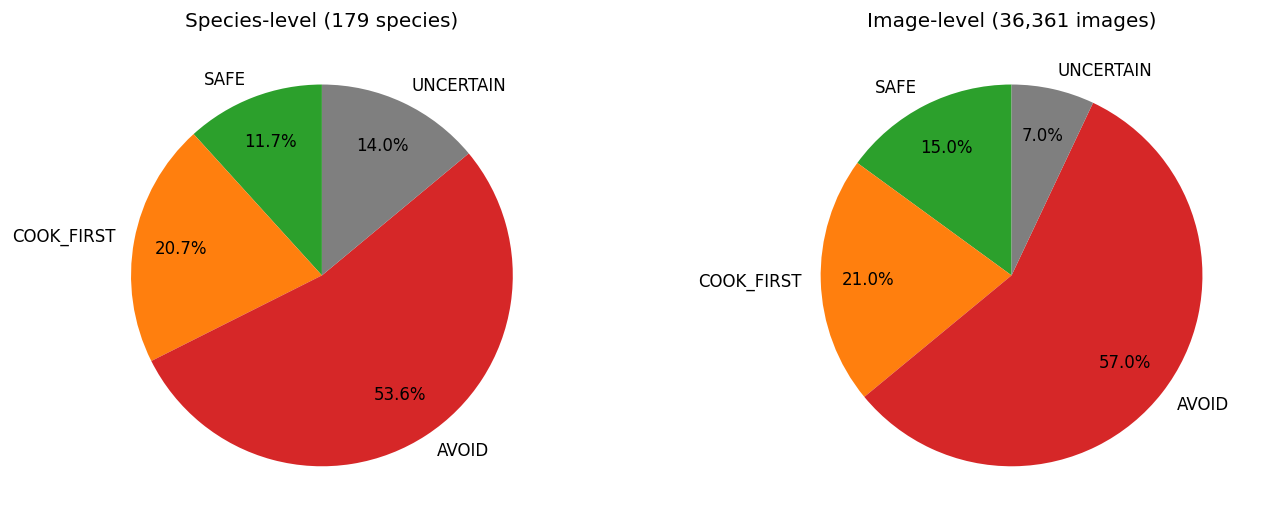
\includegraphics[width=0.95\linewidth]{results/figures/species_vs_image_bucket_pie.png}
\caption{Bucket distribution at the species level (left) and the image level
(right). The image-level view is what the classifier actually sees and is
substantially more balanced than the raw species distribution.}
\label{fig:bucket-pie}
\end{figure}

The per-genus composition (Figure~\ref{fig:genus-bucket}) shows that the
six genera present qualitatively different sub-problems. \emph{Mycena} is
uniformly AVOID and is therefore trivial at the bucket level even when
species-level accuracy is poor. \emph{Boletus} is split only between SAFE
and COOK\_FIRST, again easy at the bucket level. The remaining four genera
(\emph{Agaricus}, \emph{Amanita}, \emph{Clitocybe}, \emph{Russula}) are
$3$- or $4$-way mixtures, and \emph{Russula} alone contributes $16$ of the
$25$ UNCERTAIN species. The \emph{Amanita} entry is the most safety-critical:
$9$ of its $17$ species map to AVOID and include the deadliest taxa in the
dataset.

\begin{figure}[h]
\centering
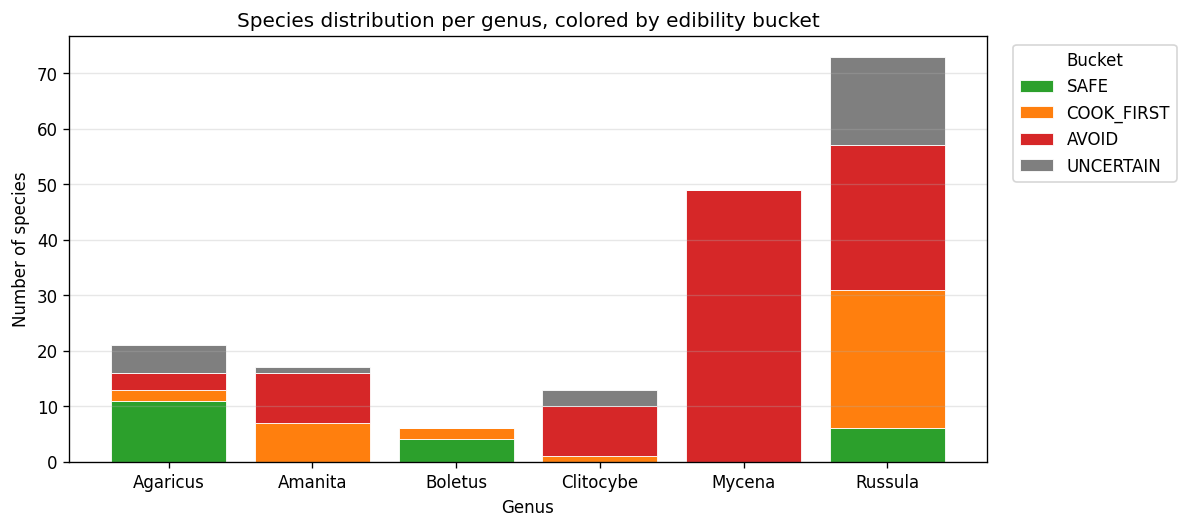
\includegraphics[width=0.85\linewidth]{results/figures/species_per_genus_bucket.png}
\caption{Number of species per genus, coloured by edibility bucket. \emph{Mycena}
is uniformly AVOID; \emph{Russula} is the dominant contributor to UNCERTAIN;
\emph{Amanita} concentrates AVOID risk.}
\label{fig:genus-bucket}
\end{figure}

The internal composition of the AVOID bucket is heterogeneous: $52$ species
are flagged \emph{poisonous}, $42$ are \emph{inedible}, and only $2$ are
\emph{deadly}; on the LLM toxicity scale the counts are $43$ at level~1,
$46$ at level~2, $5$ at level~3, and $2$ at level~5. AVOID therefore
combines emergency-level danger with mere unpalatability and could be split
further if a future deployment wants differential warnings.

The LLM confidence distribution (Figure~\ref{fig:confidence-bucket})
validates UNCERTAIN as a genuine epistemic category rather than a dumping
ground: $96\%$ of UNCERTAIN species came back with the LLM's \emph{low}
confidence flag, while $81\%$ of SAFE species came back as \emph{high} and
no SAFE species was rated \emph{low}. The agreement between the bucket and
the confidence label is what we wanted before treating UNCERTAIN as a
research signal.

\begin{figure}[h]
\centering
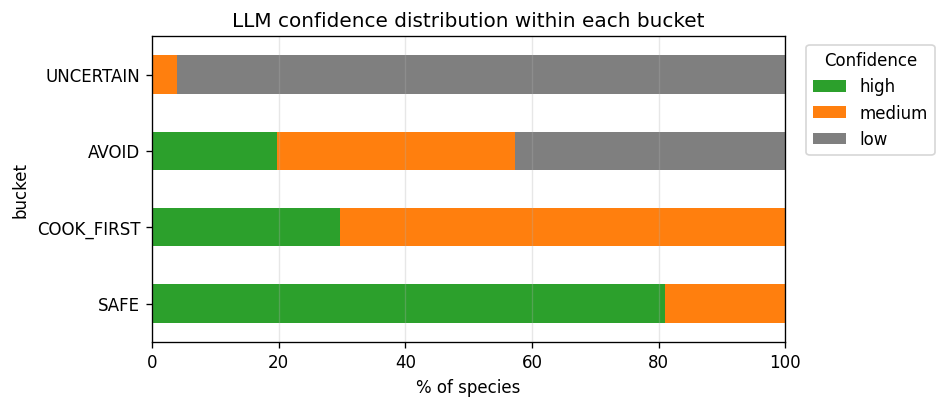
\includegraphics[width=0.7\linewidth]{results/figures/confidence_per_bucket.png}
\caption{LLM confidence within each bucket. UNCERTAIN is dominated by
\emph{low} confidence and SAFE by \emph{high}, supporting the use of
UNCERTAIN as a distinct epistemic category.}
\label{fig:confidence-bucket}
\end{figure}

\subsection{Embedding Sanity Check and Full-Supervision Ceiling}

Loading the public DF20M ViT-B/16-224 checkpoint and extracting
$\ell_2$-normalized $768$-dimensional features takes about $20$ minutes for
the full $36{,}361$ images on Apple Silicon (MPS). A logistic regression
fit on these features reaches $0.981$ train and $\textbf{0.626}$ test
species accuracy, in the $0.60$--$0.72$ range we expected from the original
backbone~[1]. This rules out a checkpoint-loading bug and confirms that the
embedding space already carries most of the species signal.

Training the MC-dropout MLP head on the entire labeled pool ($32{,}724$
images) gives the full-supervision ceiling reported in
Table~\ref{tab:ceiling}. Bucket accuracy is high in absolute terms but the
per-bucket recall is very uneven: AVOID is recovered at $0.895$ while
UNCERTAIN sits at only $0.535$. This $0.36$ gap is the headroom that
strategy choice will be measured against in Section~5.4. Soft decoding
(Equation~\ref{eq:soft}) lifts overall accuracy by $0.7$ points and AVOID
recall by $1.2$ points, but actually loses $0.8$ points on UNCERTAIN, which
foreshadows the trade-off discussed below.

\begin{table}[h]
\centering
\small
\caption{Full-supervision ceiling on the $3{,}637$-image test set.}
\label{tab:ceiling}
\begin{tabular}{lcc}
\toprule
Metric & Hard decoding & Soft decoding \\
\midrule
Species top-1 accuracy & $0.607$ & --- \\
Species macro F1       & $0.484$ & --- \\
Bucket accuracy        & $0.824$ & $0.831$ \\
Bucket macro F1        & $0.744$ & $0.750$ \\
Recall, SAFE           & $0.800$ & $0.797$ \\
Recall, COOK\_FIRST    & $0.742$ & $0.750$ \\
Recall, AVOID          & $0.895$ & $0.907$ \\
Recall, UNCERTAIN      & $0.535$ & $0.528$ \\
\bottomrule
\end{tabular}
\end{table}

\subsection{Active Learning Strategies and Learning Curves}

We ran the six query strategies for $47$ rounds each, going from
$N_{\text{init}}=400$ to $N_{\max}=5{,}000$ labels in batches of $B=100$
across five random seeds (a total of $30$ trajectories). The learning
curves under hard decoding are shown in
Figure~\ref{fig:learning-curves-hard}; the soft-decoding version
(Figure~\ref{fig:learning-curves-soft}) has the same shape, shifted
upward by roughly one point.

\begin{figure}[h]
\centering
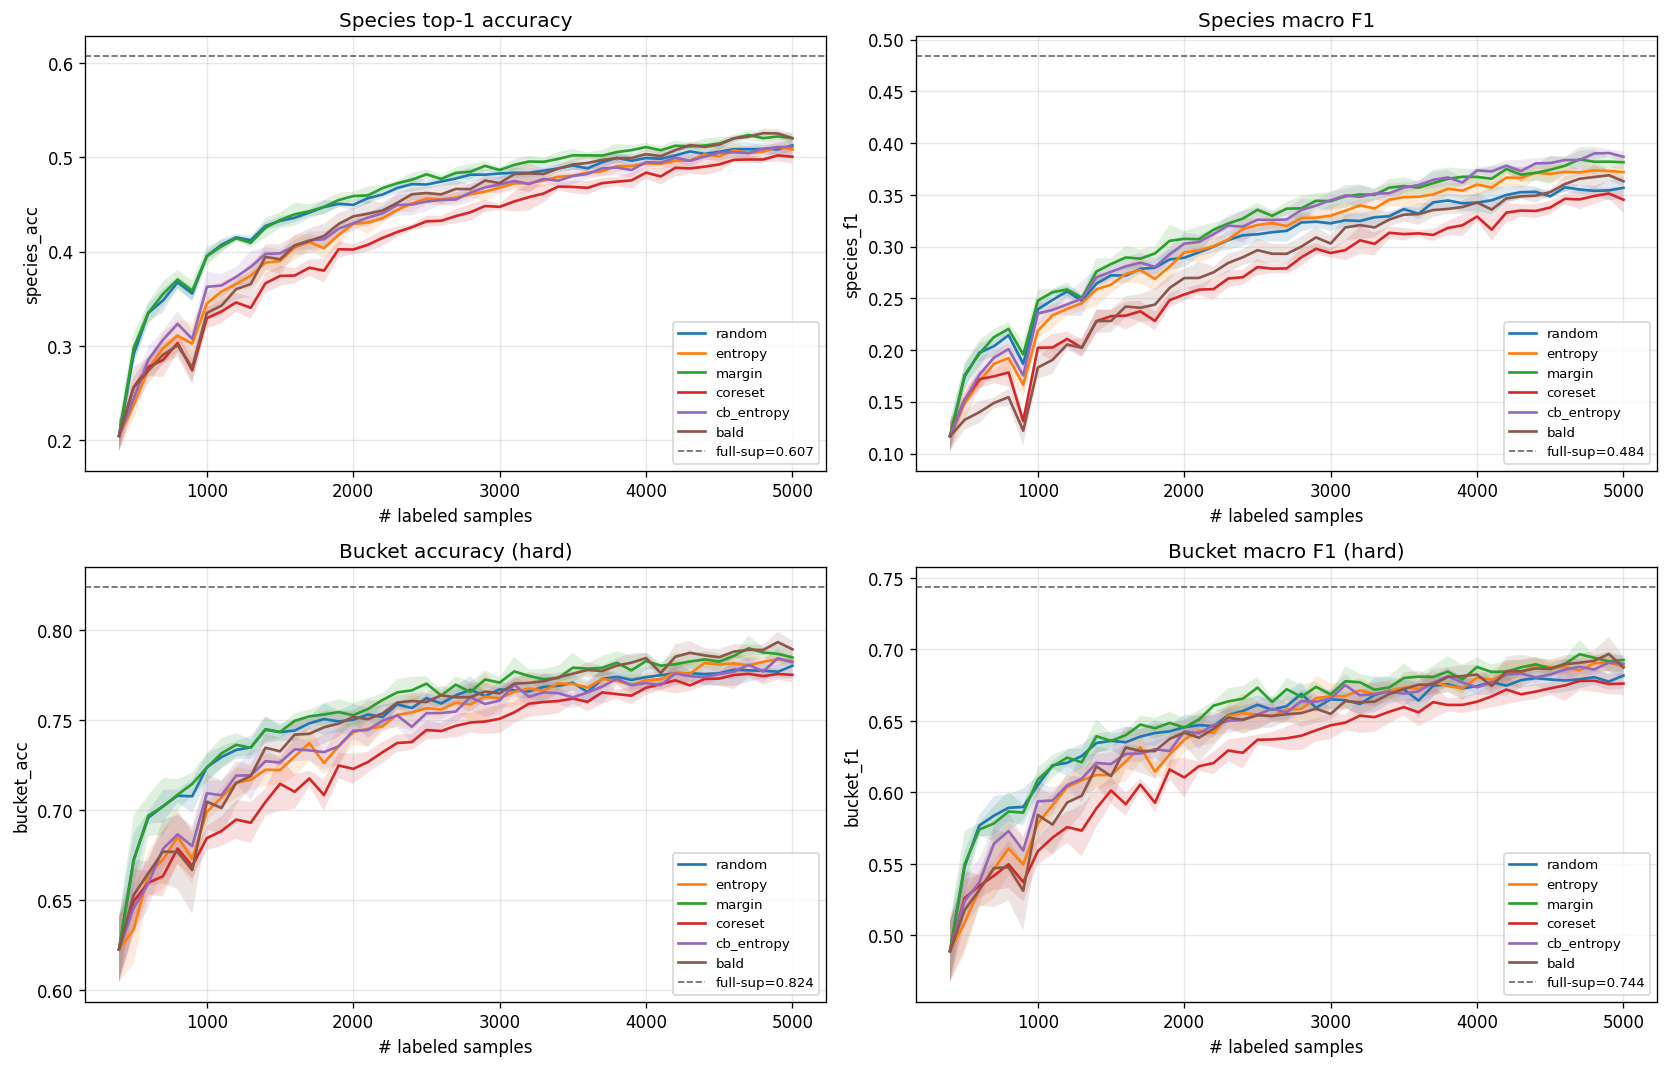
\includegraphics[width=0.95\linewidth]{results/picekvit_learning_curves_hard.png}
\caption{Learning curves for the six AL strategies under hard decoding,
mean over five seeds with $\pm 1$ standard deviation as a shaded band. The
dashed horizontal line is the full-supervision ceiling. Margin and BALD
both reach $95\%$ of the ceiling well before the $5{,}000$-label budget
runs out; core-set never closes the gap.}
\label{fig:learning-curves-hard}
\end{figure}

\begin{figure}[h]
\centering
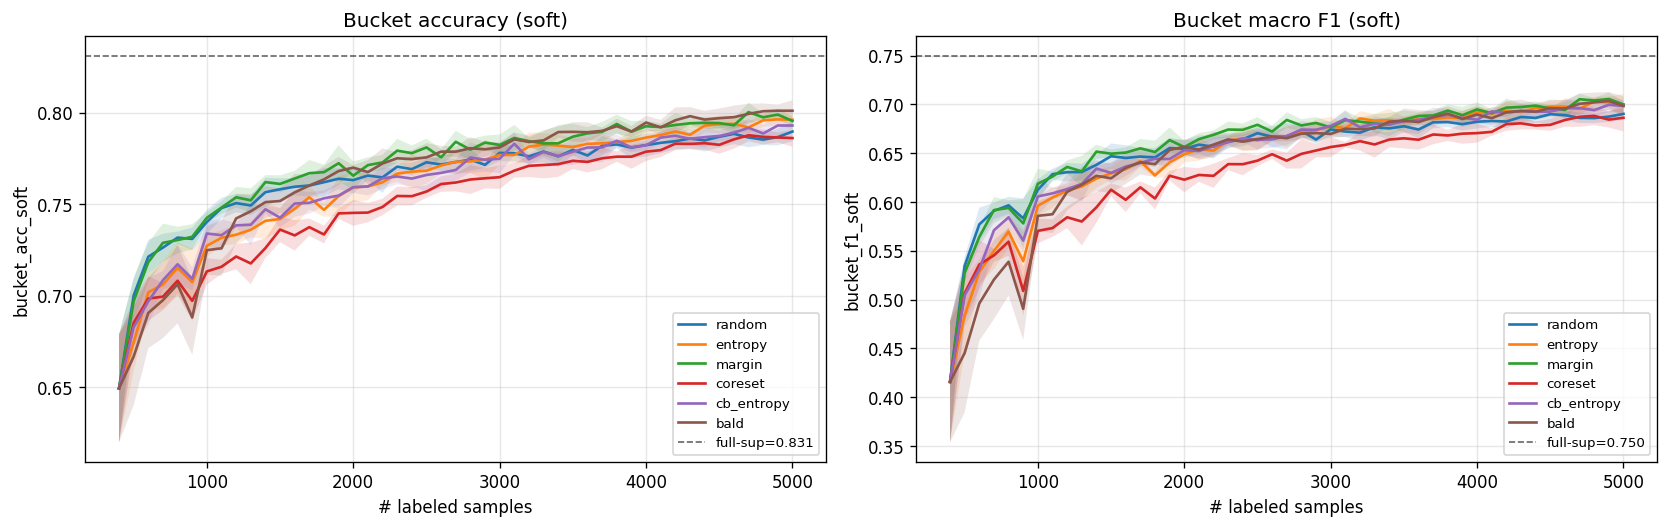
\includegraphics[width=0.95\linewidth]{results/picekvit_learning_curves_soft.png}
\caption{Learning curves under soft decoding. Soft aggregation lifts every
strategy by roughly one point on bucket accuracy and bucket macro F1.}
\label{fig:learning-curves-soft}
\end{figure}

Final-round numbers at $5{,}000$ labels are reported in
Table~\ref{tab:final-summary}. Bucket accuracy is tightly clustered: the
spread between the best (BALD, $0.789$) and the worst (core-set, $0.775$)
is only $1.4$ points, and all six strategies are within $0.6$ points of the
random baseline. Species accuracy and macro F1 tell the same story.

\begin{table}[h]
\centering
\small
\caption{Final-round metrics at $5{,}000$ labels (mean $\pm$ std over
five seeds, hard decoding). Best per column in bold.}
\label{tab:final-summary}
\begin{tabular}{lcccccc}
\toprule
Strategy & Sp.~acc & Sp.~F1 & Bk.~acc & Bk.~F1 & R$_{\text{AVOID}}$ & R$_{\text{UNC}}$ \\
\midrule
Random      & $0.513$ & $0.357$ & $0.780$ & $0.682$ & $0.876$ & $0.461$ \\
Entropy     & $0.508$ & $0.372$ & $0.783$ & $0.688$ & $0.875$ & $0.477$ \\
Margin      & $\mathbf{0.520}$ & $0.382$ & $0.785$ & $\mathbf{0.693}$ & $0.877$ & $0.487$ \\
Core-set    & $0.501$ & $0.345$ & $0.775$ & $0.676$ & $0.866$ & $0.446$ \\
CB-entropy  & $0.511$ & $\mathbf{0.387}$ & $0.782$ & $0.690$ & $0.875$ & $\mathbf{0.489}$ \\
BALD        & $\mathbf{0.520}$ & $0.363$ & $\mathbf{0.789}$ & $0.687$ & $\mathbf{0.896}$ & $0.450$ \\
\midrule
Full-sup ceiling & $0.607$ & $0.484$ & $0.824$ & $0.744$ & $0.895$ & $0.535$ \\
\bottomrule
\end{tabular}
\end{table}

\subsection{Label Efficiency Against the Full-Supervision Ceiling}

Table~\ref{tab:label-eff} reports the smallest budget at which each
strategy first crosses $80\%$, $90\%$, and $95\%$ of the full-supervision
hard bucket accuracy ($0.824$). Four observations stand out. First, every
strategy reaches the $80\%$ bar within $660$ labels, which is about $2\%$
of the training pool. Second, at the $90\%$ bar margin is the most
efficient ($1{,}340$ labels), nearly halving the requirement of core-set
($2{,}500$ labels). Third, at the $95\%$ bar the ranking shifts: margin
($3{,}700$) and BALD ($3{,}920$) both reach the target with all five
seeds, while random reaches it with only $2/5$ and core-set never reaches
it within the budget. Fourth, taking the soft-decoding view at $95\%$
(target $0.790$) makes BALD and margin tie at $3{,}360$ labels, the lowest
in the table. The corresponding bar chart is shown in
Figure~\ref{fig:label-eff}.

\begin{table}[h]
\centering
\small
\caption{Labels needed to reach $\tau$ times the full-supervision ceiling.
Cells show the mean budget across seeds, with the success rate
(seeds-reached / 5) when not all seeds succeed.}
\label{tab:label-eff}
\begin{tabular}{lcccccc}
\toprule
Target (hard, $\tau=$) & Random & Entropy & Margin & Core-set & CB-ent & BALD \\
\midrule
$80\%$ ($0.659$) & $520$ & $620$ & $\mathbf{520}$ & $660$ & $660$ & $560$ \\
$90\%$ ($0.741$) & $1400$ & $1940$ & $\mathbf{1340}$ & $2500$ & $1980$ & $1660$ \\
$95\%$ ($0.783$) & $4550$ ($2/5$) & $4500$ & $\mathbf{3700}$ & N/A & $4800$ ($4/5$) & $3920$ \\
\midrule
$95\%$ soft ($0.790$) & $4600$ ($4/5$) & $3920$ & $\mathbf{3360}$ & $4550$ ($2/5$) & $4000$ & $\mathbf{3360}$ \\
\bottomrule
\end{tabular}
\end{table}

\begin{figure}[h]
\centering
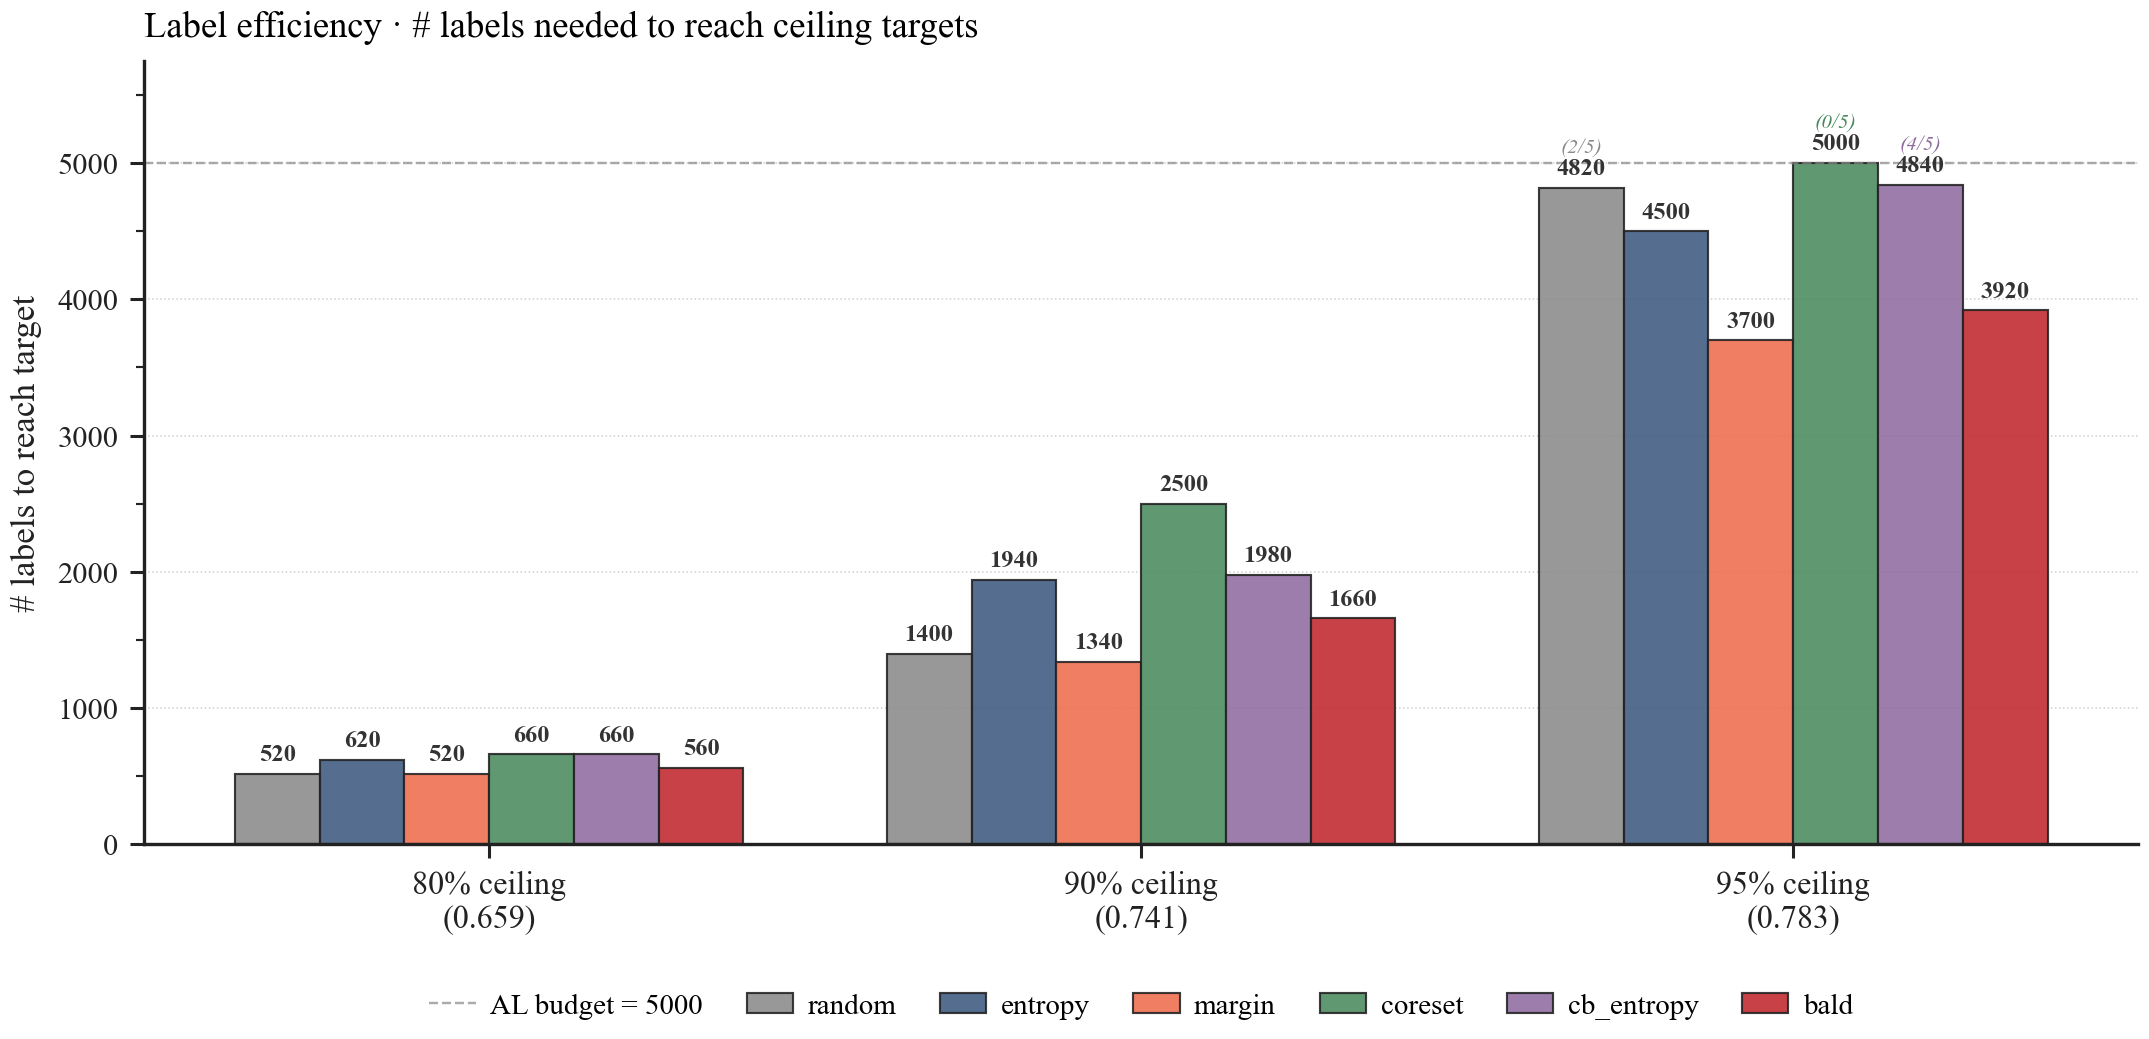
\includegraphics[width=0.85\linewidth]{results/fig_label_efficiency.png}
\caption{Labels needed to reach $80\%$, $90\%$, and $95\%$ of the
full-supervision hard bucket accuracy. Margin and BALD are consistently
the most label-efficient.}
\label{fig:label-eff}
\end{figure}

\subsection{Per-Bucket Recall and the Safety Trade-Off}

Bucket-level accuracy hides where each strategy spends its budget.
Figure~\ref{fig:bucket-recall} reports the four per-bucket recall curves.
The AVOID curves are tightly clustered around the ceiling, which is the
result we want from a safety perspective. The UNCERTAIN curves, in
contrast, are noticeably more dispersed and are still climbing at the end
of the budget for several strategies, so the choice of strategy matters
most precisely for the bucket whose label is ``do not eat; flag for
research''.

\begin{figure}[h]
\centering
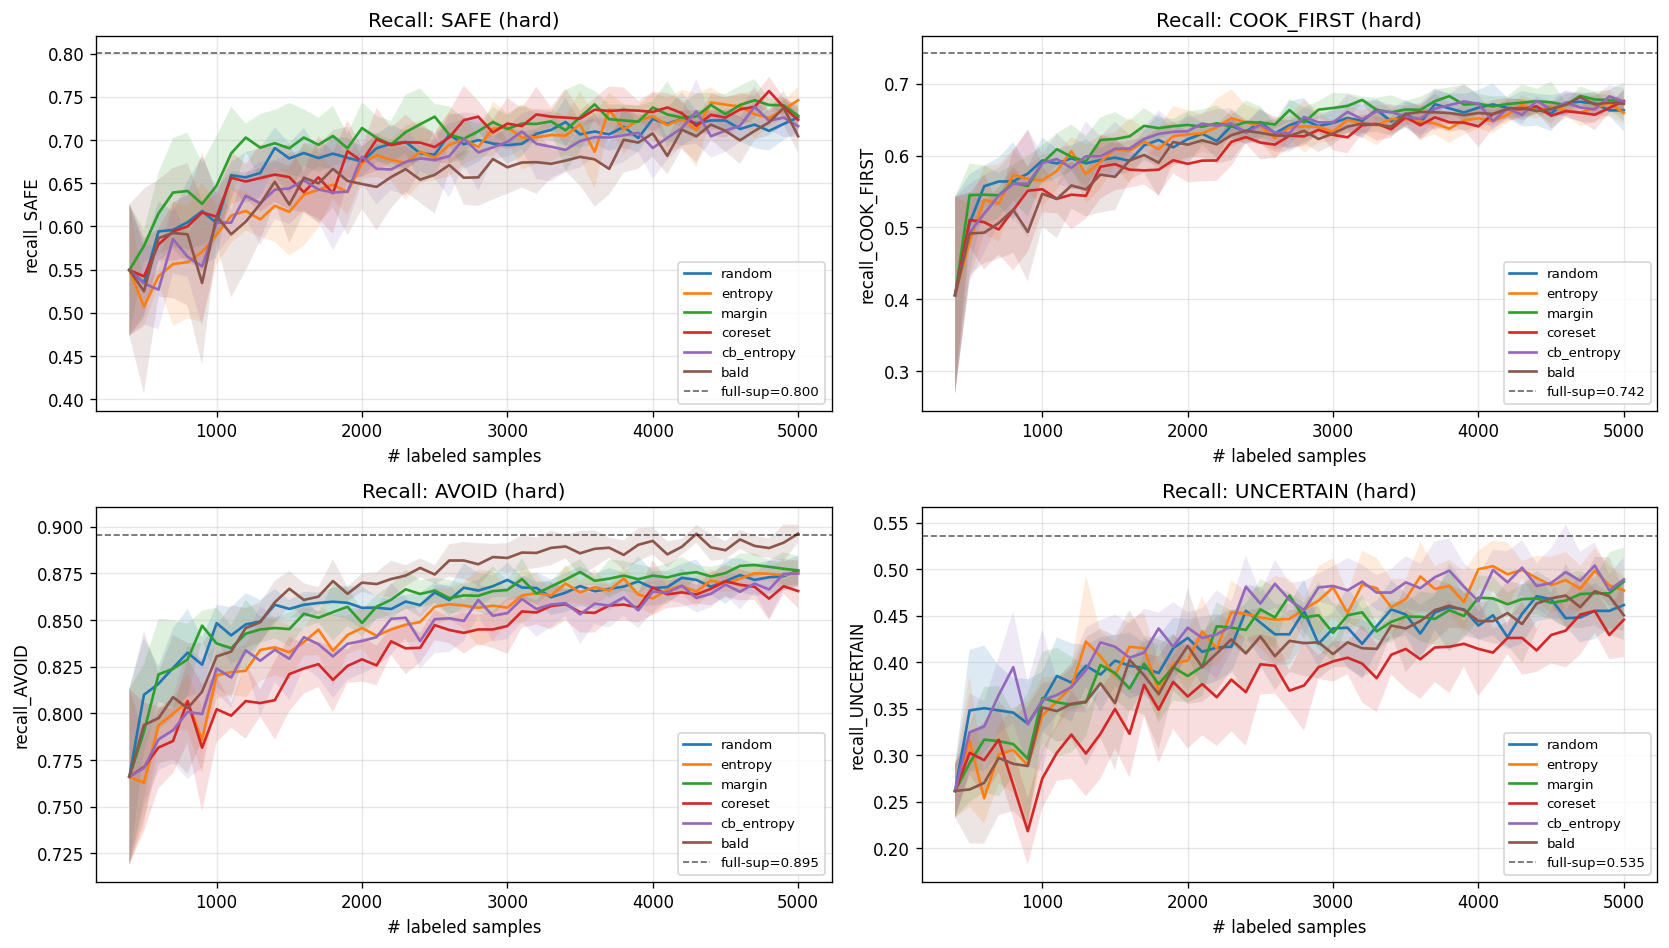
\includegraphics[width=0.95\linewidth]{results/picekvit_per_bucket_recall.png}
\caption{Per-bucket recall as a function of the label budget. AVOID
(bottom-left) is recovered uniformly across strategies; UNCERTAIN
(bottom-right) is the bucket where strategy choice matters most.}
\label{fig:bucket-recall}
\end{figure}

The Pareto plot of bucket accuracy against UNCERTAIN recall at the final
budget (Figure~\ref{fig:pareto}) makes the trade-off explicit. BALD is the
top-right corner on bucket accuracy ($0.789$) but only fifth on UNCERTAIN
recall ($0.450$); class-balanced entropy is the mirror image, top on
UNCERTAIN recall ($0.489$) but third on bucket accuracy. Margin sits on
the Pareto frontier between the two. The gap to the UNCERTAIN ceiling
ranges from $0.046$ (CB-entropy) to $0.090$ (core-set), so the choice of
strategy can move the safety-relevant recall by up to four points.

\begin{figure}[h]
\centering
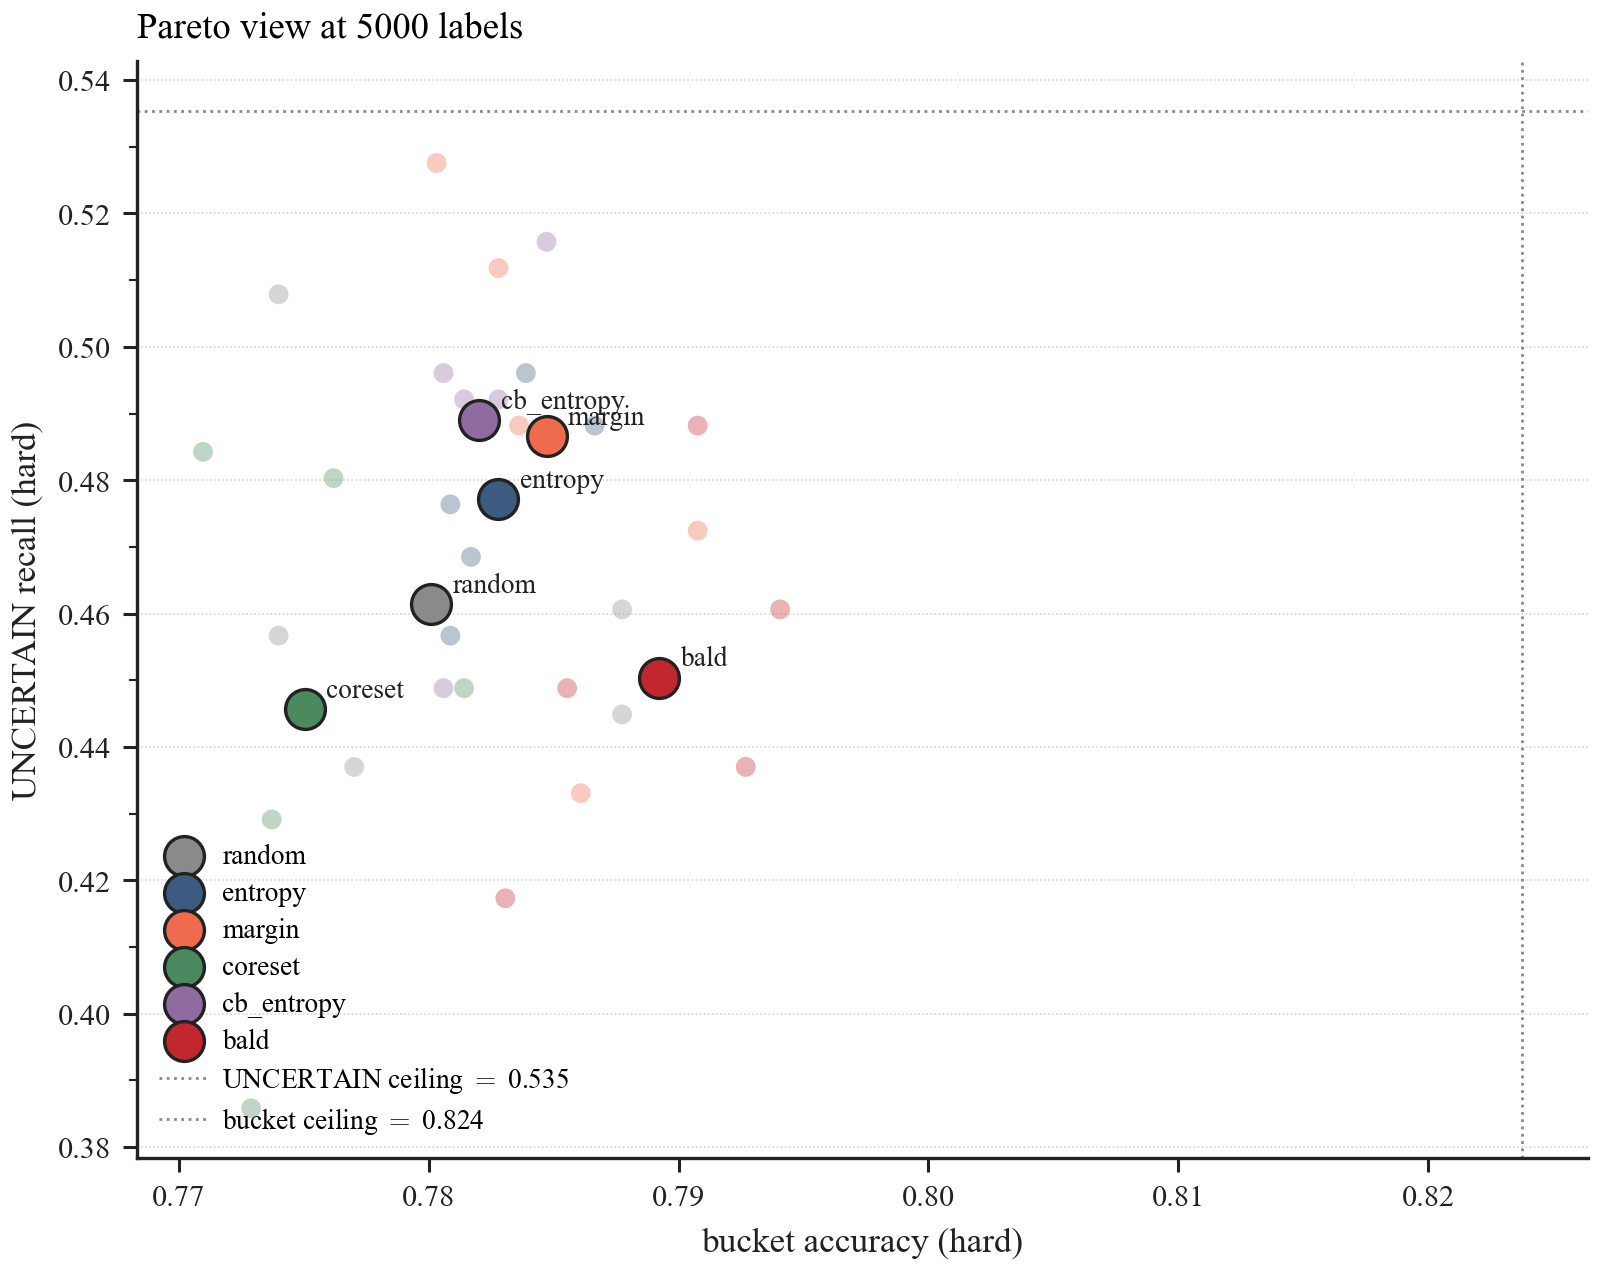
\includegraphics[width=0.7\linewidth]{results/fig8_uncertain_pareto.png}
\caption{Pareto plot of bucket accuracy versus UNCERTAIN recall at
$5{,}000$ labels. BALD optimises overall accuracy, class-balanced entropy
optimises UNCERTAIN recall, and margin sits on the frontier.}
\label{fig:pareto}
\end{figure}

\subsection{Per-Genus Analysis}

Table~\ref{tab:genus} reports per-genus species accuracy at the final
budget. The genera order roughly by visual difficulty rather than by
strategy: \emph{Boletus} and \emph{Amanita} are the easiest (mean over
strategies $\approx 0.65$), then \emph{Clitocybe} and \emph{Mycena}
($\approx 0.57$ and $0.52$), and finally \emph{Agaricus} and \emph{Russula}
($\approx 0.47$ and $0.42$). The strategy ranking inside each genus is
narrow ($\le 0.06$), which means the headline differences between
strategies do not come from any one genus.

The most important per-genus result for the safety story concerns
\emph{Amanita}, the lethal genus. Although species-level accuracy on
\emph{Amanita} only reaches $0.65$, the soft-aggregated AVOID recall on
\emph{Amanita} is $0.904$ and the COOK\_FIRST recall is $0.819$ (from the
genus-bucket breakdown). In other words, even when the model cannot name
the exact \emph{Amanita} species, the bucket-level decoder still puts
roughly nine out of ten lethal specimens into AVOID. The benefit of the
species-then-aggregate decoder in Equation~\eqref{eq:soft} is most visible
on this genus.

\begin{table}[h]
\centering
\small
\caption{Per-genus species accuracy at $5{,}000$ labels (mean over five
seeds).}
\label{tab:genus}
\begin{tabular}{lcccccc}
\toprule
Strategy & Agaricus & Amanita & Boletus & Clitocybe & Mycena & Russula \\
\midrule
Random     & $0.459$ & $\mathbf{0.667}$ & $0.664$ & $0.557$ & $0.517$ & $0.414$ \\
Entropy    & $0.464$ & $0.647$ & $0.601$ & $0.558$ & $0.508$ & $0.427$ \\
Margin     & $\mathbf{0.482}$ & $0.651$ & $0.657$ & $0.576$ & $\mathbf{0.527}$ & $0.425$ \\
Core-set   & $0.466$ & $0.617$ & $\mathbf{0.665}$ & $0.554$ & $0.507$ & $0.406$ \\
CB-entropy & $0.471$ & $0.620$ & $0.625$ & $0.542$ & $0.526$ & $\mathbf{0.431}$ \\
BALD       & $0.446$ & $\mathbf{0.674}$ & $0.656$ & $\mathbf{0.601}$ & $0.508$ & $0.437$ \\
\bottomrule
\end{tabular}
\end{table}

\begin{figure}[h]
\centering
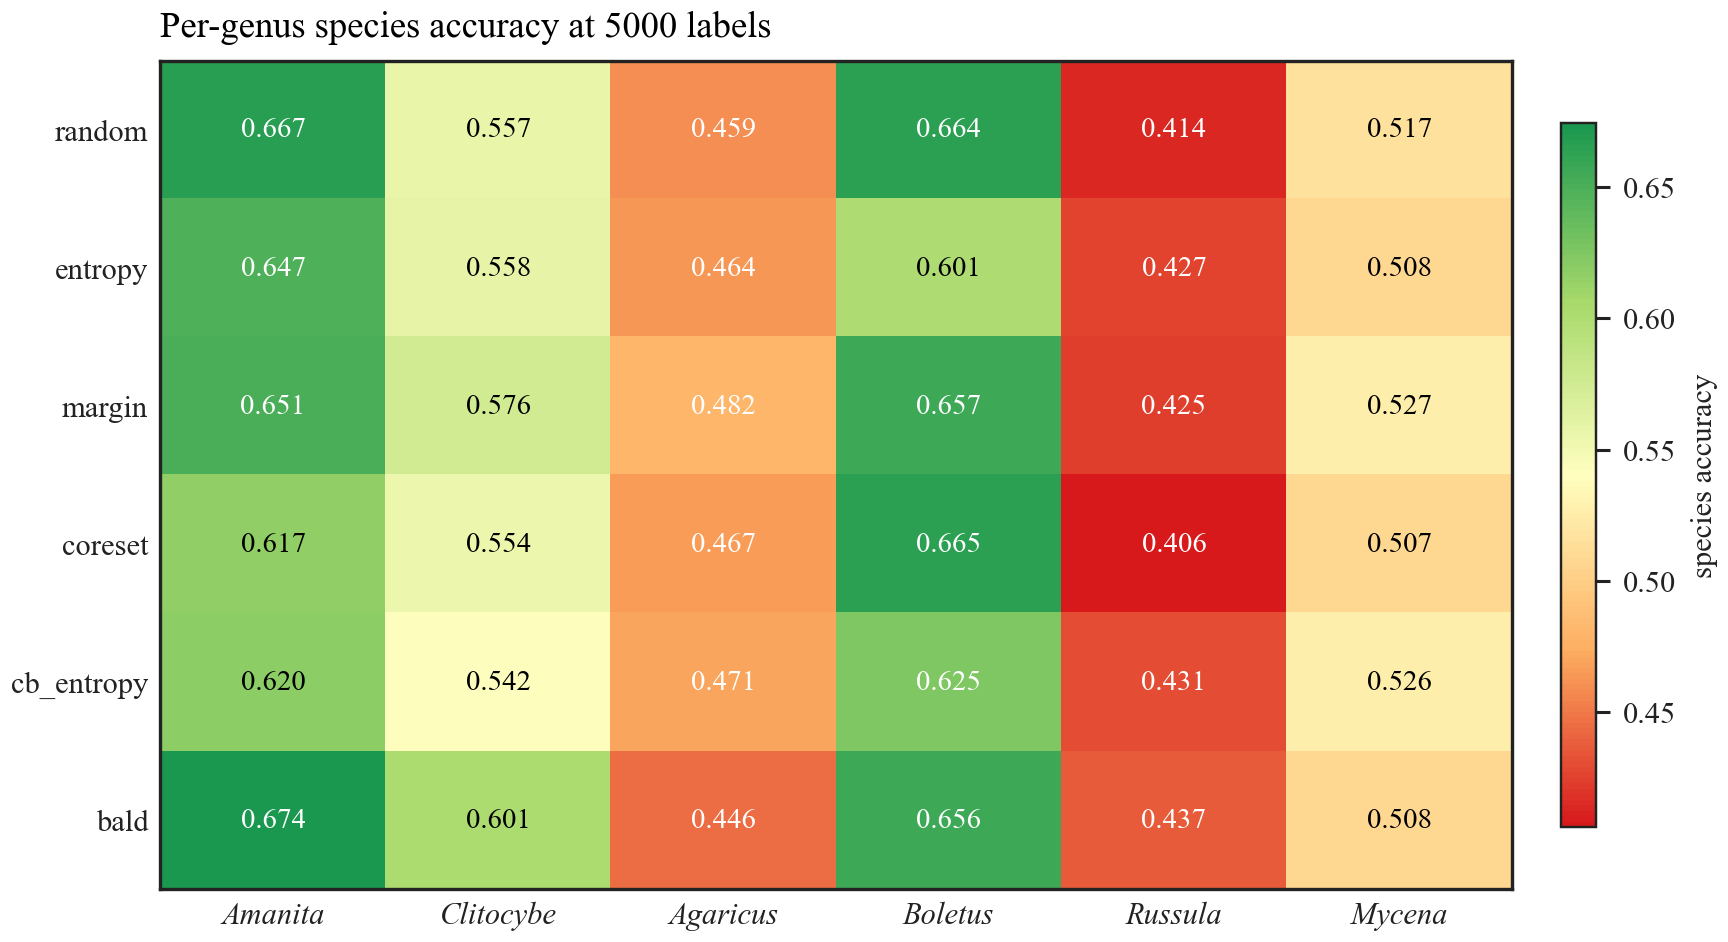
\includegraphics[width=0.9\linewidth]{results/fig11_per_genus_heatmap.png}
\caption{Per-genus, per-bucket recall heatmap. \emph{Amanita}'s AVOID row
($0.89$) is the safety-critical cell and is reached even though its
species accuracy is only $0.65$.}
\label{fig:genus-heatmap}
\end{figure}

% =====================================================
% 6. DISCUSSION
% =====================================================
\section{Discussion}

\subsection{Soft Decoding Forgives Within-Bucket Confusion}

The systematic gain from hard to soft decoding ($+0.7$ points on bucket
accuracy and a much larger swing on the per-genus AVOID recall for
\emph{Amanita}) confirms our motivating intuition: training on $179$
species and aggregating only at the end is more robust than collapsing the
labels first. The model is allowed to be confused between two
\emph{Boletus} edibles or two \emph{Amanita} toxics, as long as both
candidates fall inside the same bucket. The one bucket that does not
benefit from soft decoding is UNCERTAIN, which is consistent with its
within-bucket members being scattered across genera (mostly \emph{Russula}
plus a few \emph{Agaricus} and \emph{Clitocybe}); summing probabilities
across visually unrelated species does not help it.

\subsection{No Single AL Strategy is Best on Every Metric}

The headline finding from Section~5.4 is that the six strategies are very
close on bucket accuracy ($1.4$-point spread) yet noticeably separated on
UNCERTAIN recall ($4.3$-point spread) and on label efficiency. This is the
opposite of the usual AL story, in which uncertainty methods clearly beat
random on a single overall metric. With a strong, fungi-specialised
backbone the marginal value of any one strategy is small, and the
practical question becomes \emph{which trade-off to take}, not \emph{which
strategy is best}. The Pareto plot in Figure~\ref{fig:pareto} should
therefore be read as the main takeaway, not the final-round accuracy
column.

\subsection{Why BALD Wins Overall but Loses on UNCERTAIN}

BALD targets epistemic uncertainty, that is, examples where the MC-dropout
posterior disagrees with itself. In our setting that disagreement
concentrates inside large, visually crowded clusters (the AVOID
\emph{Mycena} and \emph{Russula} species), which is why BALD reaches
$0.896$ AVOID recall, matching the full-supervision ceiling, with only
$15\%$ of the labels. The same mechanism hurts it on UNCERTAIN: those
species have only $2{,}553$ images total ($7\%$ of the pool), and the
posterior agrees that they are unfamiliar rather than disagreeing, so they
are passed over for examples from the larger AVOID pool. Class-balanced
entropy goes the other way by construction, paying for its UNCERTAIN
recall with a small drop in overall accuracy. Margin is the only strategy
that is on the frontier on both axes and is the most label-efficient at
the $90\%$ and $95\%$ targets, which makes it our recommended default if
only one strategy is to be deployed.

\subsection{Where the Headroom Actually Is}

The residual gap to the full-supervision ceiling at $5{,}000$ labels is
about $4$ points of bucket accuracy, but the gap from full-supervision to
a hypothetical perfect classifier is $17$ points. In other words, even an
unlimited annotation budget on the current pipeline leaves more headroom
than active learning could ever recover. The bottleneck is the frozen
ViT-B/16-224 representation: at $0.626$ logistic-regression species
accuracy, it is more than $0.1$ below the full-finetune number reported by
Picek et al.~[1] and well below the larger ViT-L/16-384 SOTA. Future
gains will come from training the backbone (or at least the last few
blocks) inside the AL loop, not from squeezing additional points out of
the strategy. The small spread between strategies in
Table~\ref{tab:final-summary} is direct evidence of this: when the
representation is the bottleneck, query selection has limited leverage.

\subsection{Implications for Safety-Critical Deployment}

Three results map directly onto a foraging-app deployment. First, AVOID
recall is essentially solved at $5{,}000$ labels for every strategy: the
classifier catches roughly nine out of ten toxic specimens, and that
number does not depend on which AL method was used to build the labeled
set. Second, the \emph{Amanita}-specific AVOID recall of $0.90$ under
soft decoding implies that, at this label budget, a wild-mushroom user
who is shown the predicted bucket and is told to defer when UNCERTAIN
comes up would be protected from the deadliest mistakes nine times out of
ten. Third, UNCERTAIN recall is the metric that genuinely depends on
strategy choice; if the deployment surfaces an explicit ``defer to an
expert'' channel rather than just a top-class label, picking
class-balanced entropy or margin over BALD changes how often that channel
fires by several points.

\subsection{Limitations}

We use a frozen backbone that was itself fine-tuned on the same DF20-Mini
training pool we sample from, which makes our embeddings an upper bound
on what a true cold-start AL pipeline would see. We also keep the head
small and retrain it from scratch each round, both for runtime reasons
and because warm-starting biased the BALD scores in early experiments;
we did not study fine-tuning of the backbone inside the AL loop. The
edibility labels come from a single LLM call with no expert review, and
the AVOID bucket lumps two deadly species together with $89$ merely
poisonous or inedible species. Finally, all experiments are on Danish
fungi; transfer to a new region would require both a new embedding pass
and at least a partial re-labeling of the edibility hierarchy.

% =====================================================
% REFERENCES
% =====================================================
\section*{References}

\begin{singlespace}
\small
\begin{enumerate}[leftmargin=2em,itemsep=2pt]

\item L.~Picek, M.~\v{S}ulc, J.~Matas, T.~S.~Jeppesen, J.~Heilmann-Clausen,
T.~L\ae{}ss\o{}e, and T.~Fr\o{}slev,
``Danish Fungi 2020 -- Not Just Another Image Recognition Dataset,''
in \emph{Proc.\ IEEE/CVF Winter Conf.\ on Applications of Computer Vision (WACV)},
2022, pp.\ 1525--1535.

\item L.~Picek, M.~\v{S}ulc, J.~Matas, J.~Heilmann-Clausen, T.~S.~Jeppesen, and
E.~Lind, ``Automatic Fungi Recognition: Deep Learning Meets Mycology,''
\emph{Sensors}, vol.\ 22, no.\ 2, p.\ 633, 2022.

\item B.~Settles, ``Active Learning Literature Survey,''
\emph{Computer Sciences Tech.\ Report 1648}, University of
Wisconsin--Madison, 2009.

\item O.~Sener and S.~Savarese, ``Active Learning for Convolutional Neural
Networks: A Core-Set Approach,'' in \emph{Proc.\ Int.\ Conf.\ on Learning
Representations (ICLR)}, 2018.

\item Y.~Gal, R.~Islam, and Z.~Ghahramani, ``Deep Bayesian Active Learning
with Image Data,'' in \emph{Proc.\ Int.\ Conf.\ on Machine Learning (ICML)},
2017, pp.\ 1183--1192.

\item Y.~Gal and Z.~Ghahramani,
``Dropout as a Bayesian Approximation: Representing Model Uncertainty in
Deep Learning,'' in \emph{Proc.\ Int.\ Conf.\ on Machine Learning (ICML)},
2016, pp.\ 1050--1059.

\item U.~Aggarwal, A.~Popescu, and C.~Hudelot,
``Active Learning for Imbalanced Datasets,''
in \emph{Proc.\ IEEE/CVF Winter Conf.\ on Applications of Computer Vision (WACV)},
2020, pp.\ 1428--1437.

\end{enumerate}
\end{singlespace}

\end{document}